\documentclass[11pt, oneside]{article}   	% use "amsart" instead of "article" for AMSLaTeX format
\usepackage[margin=1in]{geometry}                		% See geometry.pdf to learn the layout options. There are lots.
\geometry{letterpaper}                   		% ... or a4paper or a5paper or ... 
%\geometry{landscape}                		% Activate for rotated page geometry
%\usepackage[parfill]{parskip}    		% Activate to begin paragraphs with an empty line rather than an indent
\usepackage{graphicx}				% Use pdf, png, jpg, or eps§ with pdflatex; use eps in DVI mode
								% TeX will automatically convert eps --> pdf in pdflatex		
\usepackage{amssymb}
\usepackage{awesomebox}
%SetFonts

%SetFonts

\usepackage{amsmath}
\DeclareMathOperator{\plainmod}{\text{ mod }}
\let\emptyset\varnothing

\newcommand{\reals}{\mathbb{R}}
\newcommand{\realsText}{$\mathbb{R}$}
\newcommand{\ints}{\mathbb{Z}}
\newcommand{\intsText}{$\mathbb{Z}$}

\title{Homework 6}
\author{Discrete Structures 2}
\date{due: 20 April 2023, 8:00am}							% Activate to display a given date or no date

\begin{document}
\maketitle
%\section{}
%\subsection{}

Your task for this homework will be to answer the following questions without using any calculating resources. 
Your responses should be submitted via blackboard by the due date above as a PDF (submissions in any other format will be returned to the user and a resubmissions will be requested). 
You are free to use whatever tools you would like to generate the response document: 
scanned hand-written paper, 
tablet generated hand-written, 
microsoft word (with this option, please use the equation editor to correctly format your responses), 
\LaTeX, etc.
Your TA, IA, and Instructor are available to help during their designated office hours or via email 
(note that emails sent during non-business hours may not be responded to until the next working day). 

%\importantbox{
%\textbf{Note:} all of these questions are on topics from chapters 5; thus you will only be proving by induction in this homework assignment. 
%}
\begin{enumerate}

%11.1-3
\item Draw a graph with the following nodes and edges? 
(make sure to ask yourself the following questions: 
Does it make sense for the graph to be directed or undirected? 
Is the graph going to be simple?)
\begin{enumerate}
\item The nodes $V=\{1,2,...,10\}$; and edge connects $x$ and $y$ if the greatest common denominator of the two numbers is $1$. 
\item The nodes $V=\{1,2,...,10\}$; and edge connects $x$ and $y$ if $y$ is evenly divisible by $x$.
\item The nodes $V=\{1,2,...,10\}$; and edge connects $x$ and $y$ if $x<y$.
\end{enumerate}

%11.8
\item If $G=\langle V, E \rangle$ is an \emph{undirected}, simple graph with $n$ nodes, what is the largest $|E|$ can be? smallest? explain your answers. 
%11.9
\item If $G=\langle V, E \rangle$ is an \emph{directed}, simple graph with $n$ nodes, what is the largest $|E|$ can be? smallest? explain your answers.
%11.10
\item If $G=\langle V, E \rangle$ is an \emph{directed} graph with self-loops allowed and $n$ nodes, what is the largest $|E|$ can be? smallest? explain your answers.

\item \label{q:isomorph} Determine if the pairs of graphs in Figure~\ref{fig:isomorph} are isomorphic? 
Justify your answers. 
(note there are two pairs of graphs in the figure and thus you will be providing two answers.)
\begin{figure}
\centering
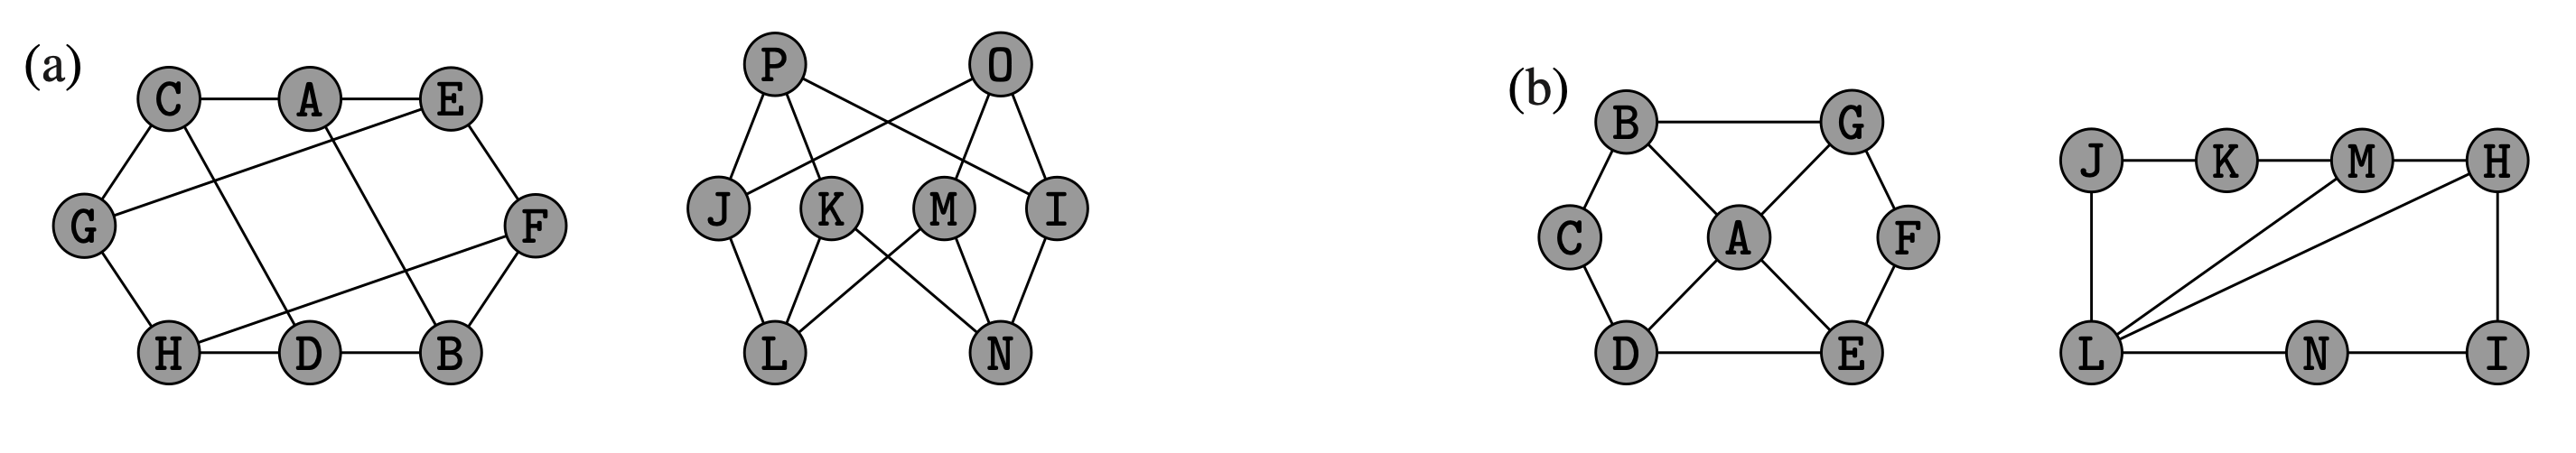
\includegraphics[width=\textwidth]{isomorph}
\caption{Graph pairs for Question~\ref{q:isomorph}.}
\label{fig:isomorph}
\end{figure}

%11.62-63
\item 
Consider a bipartite graph with a set $L$ of nodes in the left column and a set of nodes $R$ on the right column, where $|L| = |R|$. 
Prove or disprove the following claims:
\begin{enumerate}
\item The sum of the degrees of the nodes in $L$ must equal the sum of the degrees of the nodes in $R$.
\item The sum of the degrees of the nodes in $L$ must be even.
\end{enumerate}

\item \label{q:connected} Use the graphs in Figure~\ref{fig:connected} to determine the following:
\begin{enumerate}
\item Enumerated the connected components of Figure~\ref{fig:connected}a. Is the graph connected?
\item Enumerated the strongly connected components of Figure~\ref{fig:connected}b. Is the graph strongly connected?
\end{enumerate}


\begin{figure}
\centering
\begin{minipage}{.5\textwidth}
\centering
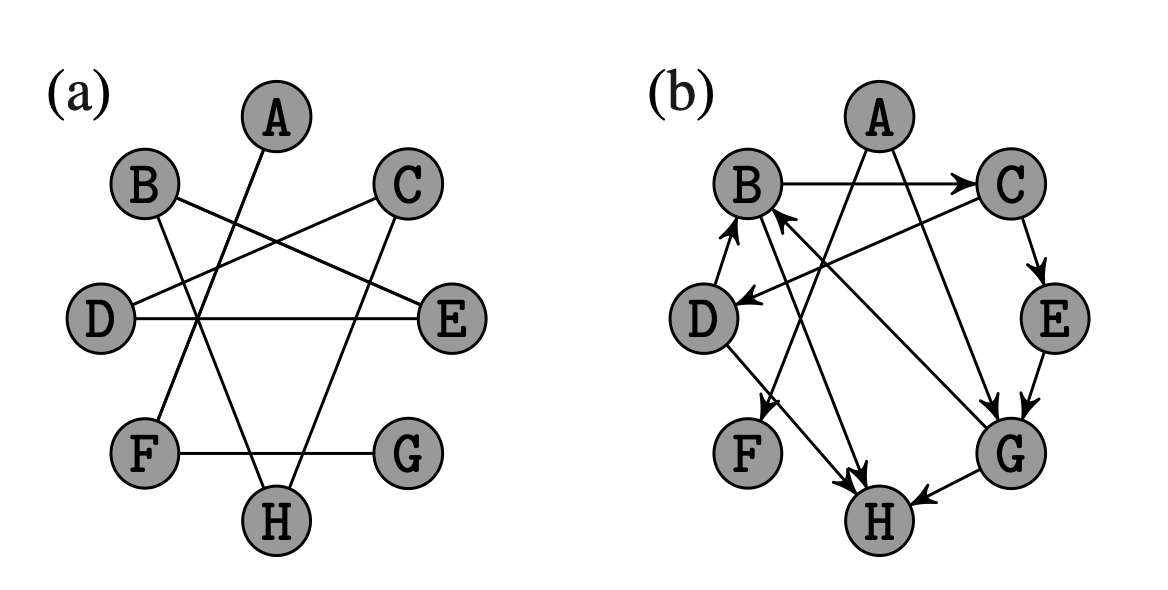
\includegraphics[width=\textwidth]{connected}
\caption{Graph pairs for Question~\ref{q:connected}.}
\label{fig:connected}
\end{minipage}%
\begin{minipage}{.5\textwidth}
\centering
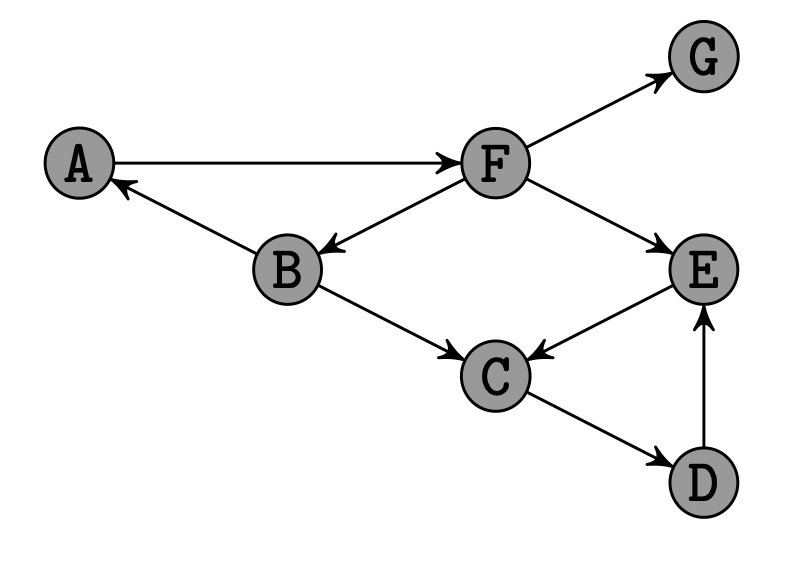
\includegraphics[width=0.65\textwidth]{BFS}
\caption{Graph pairs for Question~\ref{q:BFS}.}
\label{fig:BFS}
\end{minipage}%
\end{figure}

\item \label{q:BFS} If we run the BFS algorithm on the graph in Figure~\ref{fig:BFS} thating at each of the following nodes, what is the \emph{last} node BFS discovers. 
(if there is a tie, list all of the nodes.)
\begin{enumerate}
\item \texttt{A}
\item \texttt{B}
\item \texttt{E}
\end{enumerate}


\end{enumerate}
\end{document}